\documentclass[showpacs,twocolumn,aps,floatfix,superscriptaddress,noshowpacs]{revtex4}
\usepackage[mathlines]{lineno}% Enable numbering of text and display math

\usepackage{amsthm,amsmath,amssymb,graphicx,bm,color,mathrsfs,verbatim,epstopdf,dcolumn,dsfont,cancel}
\usepackage{ulem,cancel,comment}

\usepackage{graphicx}


%define path for figs
\graphicspath{{figs/},
		  }

\usepackage{hyperref}
\hypersetup{ 
	colorlinks   = true
}

% Use following commands if you want to see comments and deletions
\newcommand*{\red}{\textcolor{red}}
\newcommand*{\blue}{\textcolor{blue}}
\newcommand*{\green}{\textcolor{green}}
\newcommand*{\pink}{\textcolor{pink}}
\newcommand*{\cyan}{\textcolor{cyan}}

% user-defined commands come here
\newcommand{\ra}{$\rightarrow$}

\DeclareMathOperator*{\argmin}{arg\,min}
\DeclareMathOperator*{\argmax}{arg\,max}

\begin{document}
	


%\preprint{APS/123-QED}

%\title{The quantum state preparation problem is equivalent to a glass !}% 
\title{Visualizing the clustering transition using unsupervised learning}%
%\title{The Spin Glass-like Phase of Optimal Quantum Control}%

\author{Alexandre G.R. Day}
\email{agrday@bu.edu}
\affiliation{Department of Physics, Boston University, 590 Commonwealth Ave., Boston, MA 02215, USA}

\author{Pankaj Mehta}
\affiliation{Department of Physics, Boston University, 590 Commonwealth Ave., Boston, MA 02215, USA}

\begin{abstract}
We revisit the two random boolean satisfiability problems 3-SAT and XORSAT, with the latter equivalent to the $p$-spin model, using recently developed machine learning techniques. We use the non-linear embedding technique known as t-SNE to learn the local manifolds in which the solutions organize. In particular we provide a visualization of the so-called clustering transitions that are known to occur in those problems. Finally, using unsupervised clustering methods we are able to automatically extract informative quantities such as the distribution of entropy of clusters. This work highlights the potential use of common machine learning tools to study statistical physics problems.
\end{abstract} 

\date{\today}
%\keywords{Suggested keywords}
%\pacs{67.85.Pq, 71.10.Fd} 
\maketitle

Landscape induces complexity, but not always : \cite{ricci2010being}

\section{Introduction}
Machine learning is finding more and more applications in the context of physics \cite{2018arXiv180308823M}.
Chris Moore discussion, etc. cite M�zard, stat. phys. and glassy phases have been discussed in 
the context of quantum optimal control \cite{2018arXiv180310856D}.

\begin{figure}[t!]	
	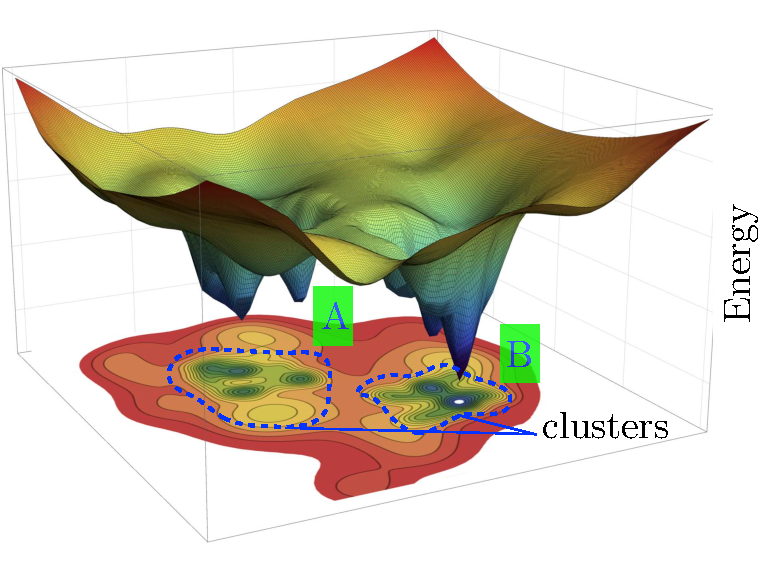
\includegraphics[width=1.0\columnwidth]{figs/rugged_vf-crop.pdf}
	\caption{\label{fig:schematic} Problem setting. (a) A complicated rugged landscape. One can visualize the low-energy local minima
	configurations as organizing into clusters. Clusters are separated by large distances and minima within a cluster are separated by small distances. In optimization or satisfiability problems
	in on a high-dimensional configurational space, clustering can be visualized using an embedding or projection to a low-dimensional space.}
\end{figure}

\begin{figure}[t!]
	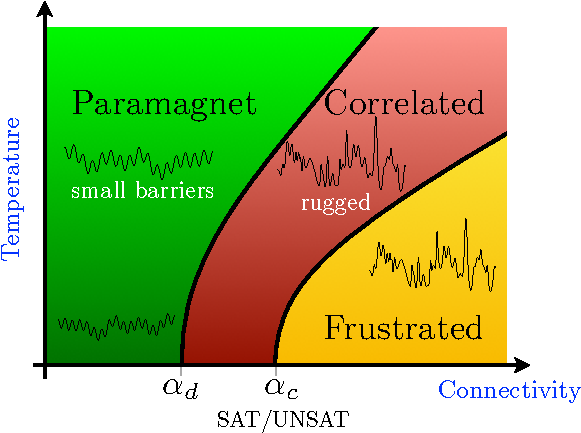
\includegraphics[width=1.0\columnwidth]{figs/cartoon_pdiag-crop.pdf}
	\caption{\label{fig:schematic2} The generic phase diagram of random satisfiability problems. By defining the energy as the number of unsatisfied clauses in a random SAT problem, one can obtain
	a temperature vs. connectivity phase diagram. The connectivity represents the average connectivity of each variable with other variables. Generically, three phases occur in such a setting: (a) Trivial phase: paramagnetic phase where the optimization is easy and the underlying landscape is nearly smooth. (b) Correlated phase: Rugged landscape analogous to a spin glass, but where the ground-state still possesses zero energy. (c) Frustrated landscape: no configuration satisfies all interactions.}
\end{figure}

\section{Model studied}
\emph{$p$-spin model}---. We consider the diluted $p$-spin model with $p=3$, defined as:
\begin{equation}
H=-\sum_{\langle ijk \rangle}^{\alpha N} J_{ijk} s_i s_j s_k, \label{pspin}
\end{equation}
where $J_{ijk}$ take value $+1$ or $-1$. An instance of the diluted $p$-spin model is obtained by choosing $\alpha N$ such couplings uniformly at random. The zero-temperature limit of the $p$-spin model
is equivalent to the $p$-XORSAT problem from computer science. The $p$-XORSAT corresponds to a linear system of equations in base 2 of the form $A\vec{x}=\vec{y}$ obtained from the mapping $s_i=(-1)^{x_i},~J_{ijk}=(-1)^{y_{ijk}}$, where $A$ is a sparse $N\times M$ matrix encoding the interactions with the $M$ constraints $\vec{y}$. As such, the problem of determining wether a XORSAT formula is satisfiable or equivalently
if the $p$-spin model possesses a non-frustrated ground-state Eq.\eqref{pspin} can be solved efficiently using Gaussian elimination which scales like $\mathcal{O}(N^3)$. The statistical properties of XORSAT have been studied using powerful methods from spin-glass physics \cite{mezard2003two}. We sampled the XORSAT solutions uniformly at random using Gaussian elimination. The results are presented in figure \ref{t-SNE}.
\\
% gaussian elimination and DPLL algorithm \cite{davis1960computing} on the reduced formulas. The results are presented in figure \ref{t-SNE}.
\emph{$k$-SAT}---.
The $k$-SAT problem blablabla 

\subsection{Method used}
\paragraph{Uniform XORSAT sampler}


\paragraph{3-SAT sampler}
Here we rely on prior work by Zecchina et al. and sophisticated implementation of decimation based survey propagation algorithm. In order to decorrelate samples as much as
possible we perform trivial isomorphism of the CNF by a permutation of the litteral's labels. However we have no theoretical guarantees that the samples obtained are uniformly
distributed in the space of 3-SAT solutions. We hope that we at least capture the clusters with the largest entropy.
\section{Results}

\begin{figure}[t!]	
	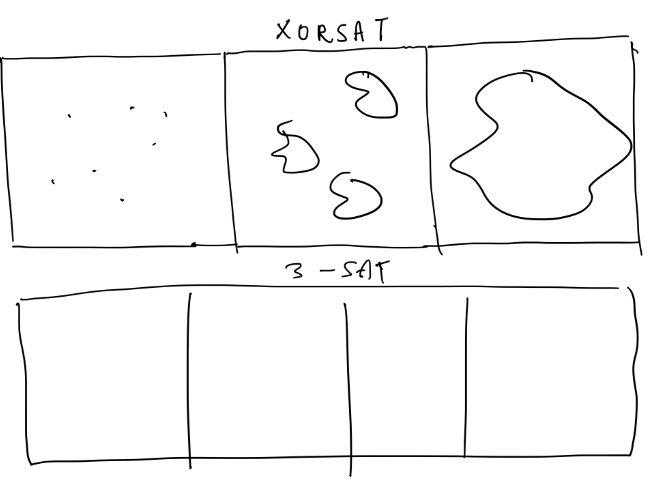
\includegraphics[width=1.0\columnwidth]{figs/fig2.png}
	\caption{\label{fig:tSNE} t-SNE visualization of the solution space as a function of the constraint parameter $\alpha$.\label{t-SNE}}
\end{figure}


\begin{figure}[t!]	
	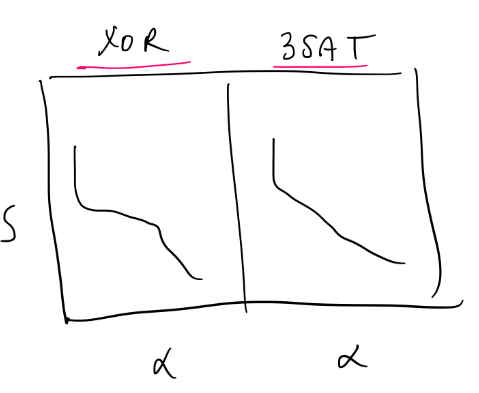
\includegraphics[width=1.0\columnwidth]{figs/fig3.png}
	\caption{\label{fig:tSNE} Entropy of clusters vs. $\alpha$.}
\end{figure}

\begin{figure}[t!]	
	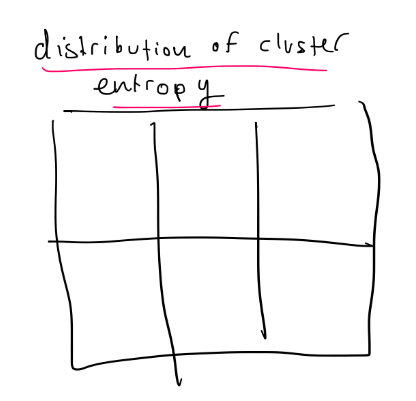
\includegraphics[width=1.0\columnwidth]{figs/fig4.png}
	\caption{\label{fig:tSNE} Distribution of cluster entropies at different $\alpha$.}
\end{figure}
\subsection{Density clustering}
Density clustering makes the intuitive assumption that clusters are high-density regions circumscribed by low-density regions in the configuration space. Density estimation is however notoriously hard in high-dimensional space due to large sampling noise. Here we use density clustering on the $t$-SNE map. This is usually sufficient to capture the main clusters in the data. Here we used a multi-scale variation of \cite{rodriguez2014clustering}, for density clustering two-dimensional data. We also made a user-friendly package for this purpose. Density estimation is done efficiently and accurately using bootstrapped kernel density estimates see Appendix \ref{dcluster}. 


\subsection{Results and Discussion}
Spin glass models such as the Sherrington-Kirkpatrick model or the Anderson model are known to be NP-complete \cite{venturelli2015quantum}. Consequently it is believed that no algorithm can be devised in order to compute the ground-state in a time scaling polynomially with the system's size. Much work has been made in trying understanding what makes a problem hard from a statistical mechanics point of view. In particular, in random satisfiability problems such $k$-SAT and XORSAT the onset of a glass transition has been associated with the appearance of frozen variables and clustering in the solution space, which has been conjectured to induce failure of local search algorithms \cite{moore2011nature}. Note that glassiness does not necessarily imply hardness to solve. Phenomenologically, it appears that for glassy problems, any local search/stochastic method will fail, i.e. finding the ground-state is exponential in the system size. However, if one is able to devise some global method based on non-local updates, then some glassy problems are known to be in $P$. This is the case for instance of XORSAT, which is equivalent to solving a linear system mod 2, and thus it can be solved efficiently using gaussian elimination \cite{ricci2010being}.
\paragraph{Clustering XORSAT, 3-SAT}
\paragraph{Entropy via density clustering}
Relation to complexity and broader applications in stat. mechanics.


\section{Conclusion}


Along with this work we provide simple python packages for the $3$-SAT sampler (wrapper) and the XORSAT sampler along with a density clustering code, all of which are available at the author's GitHub. 

\section{Acknowledgements}


%State preparation plays a quintessential role in present-day studies of quantum physics. The ability to reliably manipulate and control quantum states has proven crucial to many physical systems, from the quantum mechanical emulators ultracold atoms~\cite{bason_12,vanfrank_16,wigley_16} and trapped ions~\cite{islam_11,senko_15,jurcevic_14}, through solid-state systems like superconducting qubits~\cite{barends_16}, to nitrogen vacancy centres~\cite{zhou_17}. The non-equilibrium character of quantum state manipulation makes it a difficult and not well-understood problem of ever increasing importance to building a large-scale quantum computer~\cite{nielsen}.
%
%Analytically, state preparation has been studied using both Adiabatic Perturbation Theory~\cite{kolodrubetz_16} and Shortcuts to Adiabaticity~\cite{demirplak_03,delcampo_13,jarzynski_13,sels_16}. Unfortunately, these theories have limited application in non-integrable many-body systems, for which no exact closed-form expressions can be obtained. This motivates the development of efficient numerical algorithms, such as GRAPE~\cite{glaser_98, grape_05}, CRAB~\cite{caneva_11}, and Machine Learning~\cite{judson_92,chen_14,chen_14_ML,bukov_17RL,yang_17,dunjko_17,august_18,foesel_18,sorensen_18,zhang2018automatic}. The objective in Optimal Control theory is to find the set of controls that extremize a cost function, e.g.~ determine the optimal fidelity to prepare a target state, subject to physical and dynamical constraints. However, cost functions, usually defined on a high-dimensional space, are typically non-convex, and therefore there exist no algorithm guaranteed to find the optimal (global) solution in \emph{general}. Moreover, optimality does not automatically imply stability and robustness of the solution, which are required for experimental applications. Establishing the general limitations and constraints of quantum control is crucial for guiding the field forward.
%%Therefore, a fresh perspective on this old conundrum would be appreciated.  ?? ok maybe more enthusiasm here !
%\begin{figure}[t!]	
%	\includegraphics[width=1.0\columnwidth]{figs/schematic.png}
%	\caption{\label{fig:schematic} Problem setting. (a) A nonintegrable 1D Ising model subject to a global control transverse field $h(t)$. We focus on the family of bang-bang protocols with $h(t)$ taking values $\pm 4$. (b) Every bang-bang protocol generates an evolution from an initial to a final state from which we compute a fidelity w.r.t. the target state. For a discretization with $N_T$ time steps, there are $2^N_T$ bang-bang protocols. The set of fidelities associated to the bang-bang protocols defines a spectrum. (c) Schematic representation of a rugged fidelity landscape. (d) Moving from one protocol to another requires ``flipping" the signs of $h(t)$ at different times. }
%\end{figure}

%\emph{Model studied and methods.---}Consider quantum spin-$1/2$ degrees of freedom $S^\mu_j$ described by the Ising model with a time-dependent transverse-field (c.f. Fig \ref{fig:schematic}.a): % defined by the Hamiltonian
%\begin{equation}
%\label{eq:H}
%H(t) = -\sum_j JS^z_{j+1}S^z_j + g S^z_j + h(t)S^x_j,
%\end{equation}
%with interaction strength $J\!=\!1$ (sets the energy scale), and an external magnetic field of a static $z$-component $g\!=\!1$ and a bounded time-varying $x$-component $\vert h(t)\vert\!\leq\! 4$. The presence of the longitudinal $z$-field renders the model non-integrable at any fixed time $t$, with no known closed-form expression for the exact instantaneous eigenstates and eigenenergies. We work in a non-perturbative regime with all couplings of similar magnitude. 

\emph{Acknowlegements.---}
We thank C. Lauman and D. Sels. for insightful discussions. AD was supported by an NSERC PGS-D. AD and PM acknowledge support from Simon's Foundation through the MMLS Fellow program. The authors are pleased to acknowledge that the computational work reported on in this paper was performed on the Shared Computing Cluster which is administered by \href{https://www.bu.edu/tech/support/research/}{Boston University's Research Computing Services}. The authors also acknowledge the Research Computing Services group for providing consulting support which has contributed to the results reported within this paper.

\bibliographystyle{apsrev4-1}
\bibliography{ref}

\newpage

\begin{widetext}

\section*{\large Supplemental Material}


\section{\label{sec:densecluster} Density clustering via kernel density estimates}

\end{widetext}
\end{document}